%-------------------------
% Resume in Latex
% Author : Jake Gutierrez
% Based off of: https://github.com/sb2nov/resume
% License : MIT
%------------------------

\documentclass[letterpaper,12t]{article}

\usepackage{latexsym}
\usepackage[empty]{fullpage}
\usepackage{titlesec}
\usepackage{marvosym}
\usepackage[usenames,dvipsnames]{color}
\usepackage{verbatim}
\usepackage{enumitem}
% \usepackage[hidelinks]{hyperref}
\usepackage[colorlinks=true, urlcolor=blue, linkcolor=black]{hyperref}
\usepackage{fancyhdr}
\usepackage[english]{babel}
\usepackage{tabularx}
\input{glyphtounicode}
\usepackage{ragged2e}

\usepackage{graphicx}
\graphicspath{ {../images/} }

%----------FONT OPTIONS----------
% sans-serif
\usepackage[sfdefault]{FiraSans}
% \usepackage[sfdefault]{roboto}
% \usepackage[sfdefault]{noto-sans}
% \usepackage[default]{sourcesanspro}

% serif
% \usepackage{CormorantGaramond}
\usepackage{charter}

\usepackage[T1]{fontenc}

\renewcommand{\normalsize}{\fontsize{11}{14}\selectfont}

\usepackage{ifthen}

\pagestyle{fancy}
\fancyhf{} % clear all header and footer fields
\fancyfoot{}
\renewcommand{\headrulewidth}{0pt}
\renewcommand{\footrulewidth}{0pt}

% Adjust margins
\addtolength{\oddsidemargin}{-0.5in}
\addtolength{\evensidemargin}{-0.5in}
\addtolength{\textwidth}{1in}
\addtolength{\topmargin}{-.5in}
\addtolength{\textheight}{1.0in}

\urlstyle{same}

\raggedbottom
\raggedright
\setlength{\tabcolsep}{0in}

% Sections formatting
\titleformat{\section}{
  \vspace{-4pt}\scshape\raggedright\large
}{}{0em}{}[\color{black}\titlerule \vspace{-5pt}]

% Ensure that generate pdf is machine readable/ATS parsable
\pdfgentounicode=1

%-------------------------
% Custom commands
\newcommand{\resumeItem}[1]{
  \item \small \justifying #1 \vspace{-2pt}
}



\newcommand{\resumeSubheadingFull}[4]{
  \vspace{-2pt}\item
    \begin{tabular*}{0.97\textwidth}[t]{l@{\extracolsep{\fill}}r}
      \textbf{#1} & #2 \\ 
      \textit{\small#3} & \textit{\small #4} \\ 
    \end{tabular*}\vspace{-7pt}
}

\newcommand{\resumeSubheadingSimple}[2]{
  \vspace{-2pt}\item
    \begin{tabular*}{0.97\textwidth}[t]{l@{\extracolsep{\fill}}r}
      \textbf{#1} & #2 \\
    \end{tabular*}\vspace{-7pt}
}

\newcommand{\resumeSubheading}[4]{%
  \if\relax\detokenize{#3}\relax
    \resumeSubheadingSimple{#1}{#2}%
  \else
    \resumeSubheadingFull{#1}{#2}{#3}{#4}%
  \fi
}

\newcommand{\resumeSubSubheading}[2]{
    \item
    \begin{tabular*}{0.97\textwidth}{l@{\extracolsep{\fill}}r}
      \textit{\small#1} & \textit{\small #2} \\ 
    \end{tabular*}\vspace{-7pt}
}

\newcommand{\resumeSubHeading}[2]{
    \item
    \begin{tabular*}{0.97\textwidth}{l@{\extracolsep{\fill}}r}
      \small#1 & #2 \\ 
    \end{tabular*}\vspace{-7pt}
}

\newcommand{\resumeSubItem}[1]{\resumeItem{#1}\vspace{-4pt}}

\renewcommand\labelitemii{$\vcenter{\hbox{\tiny$\bullet$}}$}

\newcommand{\resumeSubHeadingListStart}{\begin{itemize}[leftmargin=0.15in, label={}]}
\newcommand{\resumeSubHeadingListEnd}{\end{itemize}}
\newcommand{\resumeItemListStart}{\begin{itemize}}
\newcommand{\resumeItemListEnd}{\end{itemize}\vspace{-5pt}}

%-------------------------------------------
%%%%%%  RESUME STARTS HERE  %%%%%%%%%%%%%%%%%%%%%%%%%%%%


\begin{document}

%----------HEADING----------
% \begin{tabular*}{\textwidth}{l@{\extracolsep{\fill}}r}
%   \textbf{\href{http://sourabhbajaj.com/}{\Large Sourabh Bajaj}} & Email : \href{mailto:sourabh@sourabhbajaj.com}{sourabh@sourabhbajaj.com}\\
%   \href{http://sourabhbajaj.com/}{http://www.sourabhbajaj.com} & Mobile : +1-123-456-7890 \\
% \end{tabular*}

\begin{center}
    \begin{minipage}[c]{0.17\textwidth}
        \centering
        \setlength{\fboxsep}{0.1pt}
        \setlength{\fboxrule}{2pt}
        \fbox{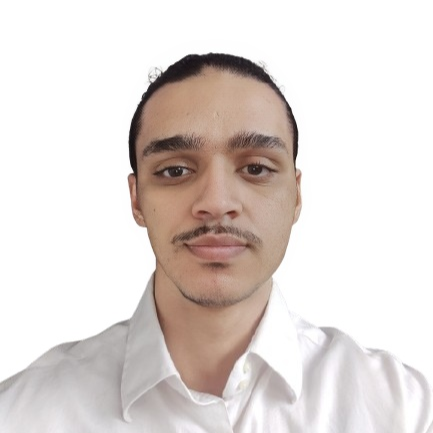
\includegraphics[width=.95\linewidth]{picture.png}}
    \end{minipage}
    \hfill
    \begin{minipage}[c]{0.8\textwidth}
        \textbf{\LARGE \scshape Moncef Bousselat}
        \vspace{3pt}
    
        \textbf{\large \scshape Ingénieur Cloud \& IA}
        \vspace{5pt}

        \begin{minipage}{\textwidth}
            \justifying \small \noindent
            Bientôt diplômé en Cloud Computing et titulaire d'un Master en Data Science et IA, 
            je recherche un poste dans le Cloud et l'IA pour mettre à profit mes 
            compétences technique et pluridisciplinaires acquises au cours de mon 
            parcours académique et professionnel.
        \end{minipage}

        \vspace{5pt}
        
        \raggedright \small 
        % \underline{Contact:}\\
        Nancy, France $|$ 
        \small +33753542166 $|$ 
        \href{mailto:a.m.bousselat@gmail.com@gmail.com}{\underline{a.m.bousselat@gmail.com}} $|$
        \href{https://www.linkedin.com/in/moncefbousselat/}{\underline{linkedin.com/in/moncefbousselat}}
        % \\

        % \underline{Links:}\\
        \href{https://github.com/Somnef}{\underline{github.com/Somnef}} $|$
        \href{https://www.somnef.com}{\underline{somnef.com}}
    \end{minipage}
\end{center}

%-----------FORMATION-----------
\section{Formation}
    \resumeSubHeadingListStart
        \resumeSubheading
        {Master en Réseaux et Cloud Computing}{Sep. 2023 -- Juil. 2025}
        {Université de Lorraine $|$ Leeds Beckett University $|$ Lulea Technical University}{Nancy, FR $|$ Leeds, UK $|$ Skelleftea, SE}
            \resumeItemListStart
                \resumeItem{Sélectionné parmi 2000+ candidats pour la bourse Erasmus Mundus "Green Networking and Cloud Computing"}
                \resumeItem{Modules clés: Services Cloud, IoT, Systèmes Robotiques Intelligents, Réseaux Sans Fil, Ingénierie des Systèmes, QoS/QoE, Analyse de Données}
            \resumeItemListEnd

        \resumeSubheading
        {Master en Science des Données et Intelligence Artificielle}{Sep. 2018 -- Juil. 2023}
        {École Nationale Polytechnique}{Alger, Algérie}
            \resumeItemListStart
                \resumeItem{Top 10\% des étudiants en classes préparatoires via concours national}
                \resumeItem{Modules clés: Bases de Données Avancées, Probabilités et Statistiques, Analyse de Données Multi-Variée, Machine/Deep Learning, TALN, Blockchain, Cloud Computing}
            \resumeItemListEnd
    \resumeSubHeadingListEnd

%-----------EXPÉRIENCE-----------
\section{Expérience}
    \resumeSubHeadingListStart
        \resumeSubheading
        {Ingénieur Cloud -- Stagiaire}{Déc. 2024 -- Juil. 2025}
        {Université de Lorraine}{Nancy, France}
            \resumeItemListStart
                \resumeItem{Développement d'un système d'identité décentralisée basé sur les Self-Sovereign Identities (SSIs) avec Hyperledger Indy}
                \resumeItem{Déploiement des agents de contrôle de la blockchain sur AWS avec Docker ECS et évaluation des performances}
            \resumeItemListEnd

        \resumeSubheading
        {Développeur Full-Stack -- Stagiaire}{Jan. 2023 -- Juil. 2023}
        {Schlumberger}{Alger, Algérie}
            \resumeItemListStart
                \resumeItem{Création d'une API REST gérant 1000+ transactions/jour sur une blockchain privée Hyperledger Fabric}
                \resumeItem{Déploiement d'une application (Flask, VueJS, Docker) sur AWS ECS, réduisant les coûts de pénalité de 75\%}
            \resumeItemListEnd

        \resumeSubheading
        {Ingénieur Data et IA -- Stagiaire}{Oct. 2022 -- Jan. 2023}
        {Ericsson}{Alger, Algérie}
            \resumeItemListStart
                \resumeItem{Entraînement d'un modèle YOLO pour l'identification d'équipements sur le terrain (précision 85\%)}
                \resumeItem{Construction d'un autoencodeur PyTorch pour débruitage d'images (précision 99\% sur MNIST)}
            \resumeItemListEnd

        \resumeSubheading
        {Data Analyst -- Stagiaire}{Mai 2022 -- Juil. 2022}
        {BH Advisory}{Alger, Algérie}
            \resumeItemListStart
                \resumeItem{Veille sur le marché des matériaux pour détecter les  tendances des prix et des stocks}
                \resumeItem{Développement de scrapers Web et tableau de bord VueJS pour visualisation automatisée}
            \resumeItemListEnd
    \resumeSubHeadingListEnd

%-----------PROJETS-----------
\section{Projets}
    \resumeSubHeadingListStart

        \resumeSubheading
        {Infrastructure auto-scalable sur AWS avec Terraform}{Jan. 2025}
        {\href{https://github.com/Somnef/d7001d-lab4}{\underline{Voir sur GitHub}}}{}
            \resumeItemListStart
                \resumeItem{Simulation d'attaques DDoS sur EC2 avec 20000+ instances/minute (JADE)}
                \resumeItem{Déploiement d'une infrastructure et auto-scalable résiliente via Terraform}
                \resumeItem{Construction d'un dashboard avec VueJS connecté à AWS SDK pour suivre CloudWatch}
            \resumeItemListEnd

        \resumeSubheading
        {Tolérance aux pannes avec Kubernetes}{Nov. 2024}
        {\href{https://github.com/Somnef/kubernetes-fault-tolerance}{\underline{Voir sur GitHub}}}{}
            \resumeItemListStart
                \resumeItem{Déploiement d'une appli Python sur un cluster Kubernetes avec un HPA pour le load balancing}
                \resumeItem{Load-testing avec requêtes cURL - Disponibilité de 99.9\% atteinte}
                \resumeItem{Monitoring des resources en temps réel via Prometheus et Grafana}
            \resumeItemListEnd

        \resumeSubheading
        {Évaluation IA de la potabilité de l'eau}{Mai 2024}
        {\href{https://github.com/Somnef/dl-water-quality}{\underline{Voir sur GitHub}}}{}
            \resumeItemListStart
                \resumeItem{Classification de l'eau via ses propriétés chimiques (90\% de précision)}
                \resumeItem{Comparaison des modèles de classification ML/DL sur différentes plages d'hyperparamètres}
            \resumeItemListEnd

        \resumeSubheading
        {Profilage énergétique GPU pour Deep Learning}{Avr. 2024}
        {\href{https://github.com/Somnef/gpu-profiling-for-dl}{\underline{Voir sur GitHub}}}{}
            \resumeItemListStart
                \resumeItem{Création d'un outil de profilage GPU pour 25+ combinaisons d'hyperparamètres de deep learning}
                \resumeItem{Évaluation d'un gain énergétique de 20\% pour une performance quasi-équivalente au modèle optimal}
            \resumeItemListEnd

        \resumeSubheading
        {Recommandation de salle via IoT}{Nov. 2023}
        {\href{https://github.com/Somnef/iot_project_app}{\underline{Voir sur GitHub}}}{}
            \resumeItemListStart
                \resumeItem{Déploiement d'une app sur EC2 pour collecte de température/bruitavec Arduino et stockage des données sur MongoDB}
                \resumeItem{Design d'un algorithme décisionnel pour recommandation de salle personnalisée aux critères de l'utilisateur}
            \resumeItemListEnd

        \resumeSubheading
        {Business Game}{Mai 2022}
        {}{}
            \resumeItemListStart
                \resumeItem{Encadrement d'une équipe de 4 développeurs afin de créer un jeu de simulation de marché multi-joueurs}
                \resumeItem{Optimisation du trafic réseau de l'application pour 12 équipes (1000+ requêtes/min en local)}
            \resumeItemListEnd

        \resumeSubheading
        {NEAT appliqué aux jeux vidéo}{Oct. 2022}
        {\href{https://github.com/Somnef/snake_neat_ai}{\underline{Voir sur GitHub}}}{}
            \resumeItemListStart
                \resumeItem{Reproduction de Snake et Flappy Bird avec Pygame}
                \resumeItem{Entraînement d'agents intelligents basés sur l'algorithme NEAT capables de surpasser les scores de tous les joueurs testés}
            \resumeItemListEnd

        \resumeSubheading
        {Simulateur 3D de feux de forêt}{Déc. 2021}
        {\href{https://github.com/Somnef/semi-empirical-wildfire-simulation}{\underline{Voir sur GitHub}} $|$ \href{https://www.researchgate.net/publication/354678516_Applying_semi-empirical_simulation_of_wildfire_on_real_world_satellite_imagery_data}{\underline{Lire sur ResearchGate}}}{}
            \resumeItemListStart
                \resumeItem{Reconstruction 3D de terrain réel via les images satellite de Google Earth Engine clusterisées avec l'algorithme k-means}
                \resumeItem{Développement d'une simulation de feu de forêts sur 100km² basée sur un modèle de cellular-automata semi-empirique}
            \resumeItemListEnd

        \resumeSubheading
        {Focus AI}{Nov. 2021}
        {\href{https://github.com/Somnef/focus-monitor-ai}{\underline{Voir sur GitHub}}}{}
            \resumeItemListStart
                \resumeItem{Détection de perte de concentration via suivi facial en temps réel avec Mediapipe}
                \resumeItem{Les tests démontrent une augmentation de 50\% de la concentration des utilisateurs}
            \resumeItemListEnd

        \resumeSubheading
        {Scraper boutique en ligne}{Avr. 2021}
        {\href{https://github.com/Somnef/CdiscountScrapper}{\underline{Voir sur GitHub}}}{}
            \resumeItemListStart
                \resumeItem{Développement de scrapers multi-sites (Amazon, CDiscount, etc.) avec suivi de prix}
                \resumeItem{Comparaison automatique avec 15\% d'économies moyennes}
            \resumeItemListEnd

    \resumeSubHeadingListEnd

%-----------PRIX & CERTIFICATIONS-----------
\section{Prix \& Certifications}
    \begin{itemize}[leftmargin=0.15in, label={}]
        \item{
            \textbf{Certifications}{: AWS Certified Solutions Architect Associate}\\
            \textbf{Prix}{: 1\textsuperscript{re} place - Arctic Challenge (Suède, 2024), 2\textsuperscript{e} place - Hackathon Google DevFest (Algérie, 2021)}\\
        }
    \end{itemize}

%-----------COMPÉTENCES-----------
\section{Compétences}
    \begin{itemize}[leftmargin=0.15in, label={}]
        \item{
        \textbf{Langages}{: Python, C/C++, Java, PHP/SQL, JavaScript/TypeScript, BASH} \\
        \textbf{Technologies}{:  NumPy, Pandas, Matplotlib, Seaborn, PyTorch, Scikit-learn, Tensorflow, Anaconda, AWS (certifié), Terraform, Docker, Kubernetes, Git, CI/CD, Prometheus, Grafana} \\
        \textbf{Langues}{: Français (C2), Anglais (C2), Arabe (natif), Suédois (notions)} \\
        }
    \end{itemize}

%-------------------------------------------
\end{document}
